\chapter{Theorie}

\section{SetlX}

\section{MNIST}

\section{Perceptrons}
Ein Perceptron ist ein mathematisches Modell zur Abbildung eines künstliches Neurons in einem Netzwerk. Es wird für die Entscheidungsfindung herangezogen, indem verschiedene Aussagen abgewägt werden. Hierbei nimmt das Perceptron eine Menge von Eingaben $x_n$ mit $n \in \{1, \cdots, n\}$ und berechnet einen einzigen binären Ausgabewert (siehe Abb. \ref{fig:perceptron}). 

\begin{figure}[hbt]
	\centering
	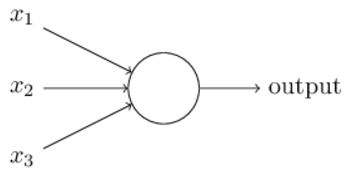
\includegraphics[scale=0.6]{Bilder/perceptron}
	\caption{Percetron mit den Eingaben $x_1, x_2, x_3$ und der Ausgabe $output$.} 
	\label{fig:perceptron} 
\end{figure}

\noindent
Für die Berechnung der Ausgabe werden sogenannte \textit{Weights} $w_n$ mit $n \in \{1, \cdots, n\}$ eingeführt, welche die Gewichtung der jeweiligen Eingabe ausdrücken. Der Ausgabewerte $output$ wird mittels der gewichteten Summe $\sum_j w_j x_k$ und einem definierten Grenzwert $threshold$ bestimmt.
\begin{equation}
	output := \left\{
	\begin{array}{ll}
 		0\ falls \sum_j w_j x_j \leq threshold \\
 		1\ falls \sum_j w_j x_j > threshold
	\end{array}\right.
\end{equation}
Werden die \textit{Weights} und der \textit{Threshold} variiert, entstehen unterschiedliche Modelle zur Entscheidungsfindung (siehe Abb. \ref{fig:perceptron_models}). Hierbei ist zu beachten, dass eine Minimierung des \textit{Thresholds} den binären Ausgabewert 1 mit einer höheren Wahrscheinlichkeit bedingt. \\


\begin{figure}[hbt]
	\centering
	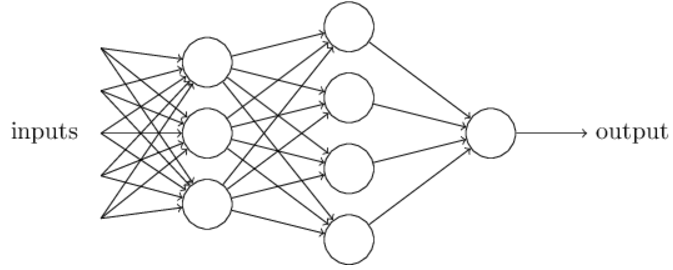
\includegraphics[scale=0.75]{Bilder/perceptron_models}
	\caption{Unterschiedliche Möglichkeiten der Entscheidungsfindung.} 
	\label{fig:perceptron_models} 
\end{figure}

\section{Sigmoid Neurons}
Für die Entwicklung lernender Algorithmen in einem Netzwerk mit Perceptrons, fällt unsere Betrachtung auf das Beispiel der Erkennung von handgeschriebenen Zahlen. Die Eingabe für das Netzwerk könnten die Raw Pixeldaten der eingescannten Bilder darstellen, welche die handgeschriebenen Zahlen abbilden. Das Ziel an dieser Stelle ist, dass das Netzwerk anhand der \textit{Weights} und \textit{Biases} lernt eine korrekte Klassifizierung der Zahlen vorzunehmen.